\documentclass[12pt,a4paper,UTF8]{ctexart}




%设置页边距
\usepackage{geometry}
\geometry{left=2.5cm,right=2.5cm,top=2.5cm,bottom=2.5cm}
\usepackage{wrapfig}



%需要用到的扩展包
\usepackage{xeCJK,amsmath,paralist,enumerate,booktabs,multirow,graphicx,float,subfig,setspace,listings,lastpage,hyperref}
\usepackage{fancyhdr}



%设置页眉页脚以及页码
\pagestyle{fancy}
\rhead{迈克尔孙干涉仪}
\lhead{大学基础物理实验报告}
\cfoot{Page\thepage/\pageref{LastPage}}
\rfoot{\today}




%报告中用到的图片存放在这个tex文件所在目录中的figures子目录中
\graphicspath{{figures/}}









%报告开始
\begin{document}
	
	
	
	
	%设置课程标题
	\begin{center}
		\heiti\LARGE{《大学基础物理实验》课程实验报告}
	\end{center}
	
	
	
	
	%设置实验人信息以及实验时间表格
	
	
	\begin{center}
		\begin{tabular}{lcr}
			
			{\songti 姓名及学号:2211082蒋丰毅}  \quad 专业:工科试验班 \quad 年级:22级 \quad 座号:10\\
			{\songti  学院:软件学院 \quad 实验组别:C组\quad 实验时间:2023年5\textbf{\textbf{\textbf{\textbf{}}}}月4日~星期五~上午}\\
			
			
		\end{tabular}
	\end{center}
	\vspace{-0.2cm}
	{\noindent}	 \rule[-10pt]{16cm}{0.05em}\\
	
	\vspace{-0.4cm}
	
	
	
	
	
	
	%实验题目
	\begin{center}
		\LARGE\textbf{迈克尔孙干涉仪}
	\end{center}
	
	
	\subsection*{[实验目的]}
    \par 1.了解迈克尔孙干涉仪的结构原理并掌握调节方法。
    \par 2.观察等厚干涉、等倾干涉。
	\par 3.测量钠双线的波长差。
	\subsection*{[实验器材]}
	\par 迈克尔孙干涉仪,光源。
\subsection*{[实验原理]}
\subsubsection*{迈克耳孙干涉仪的结构}
\begin{figure}[!htbp]
	\centering
	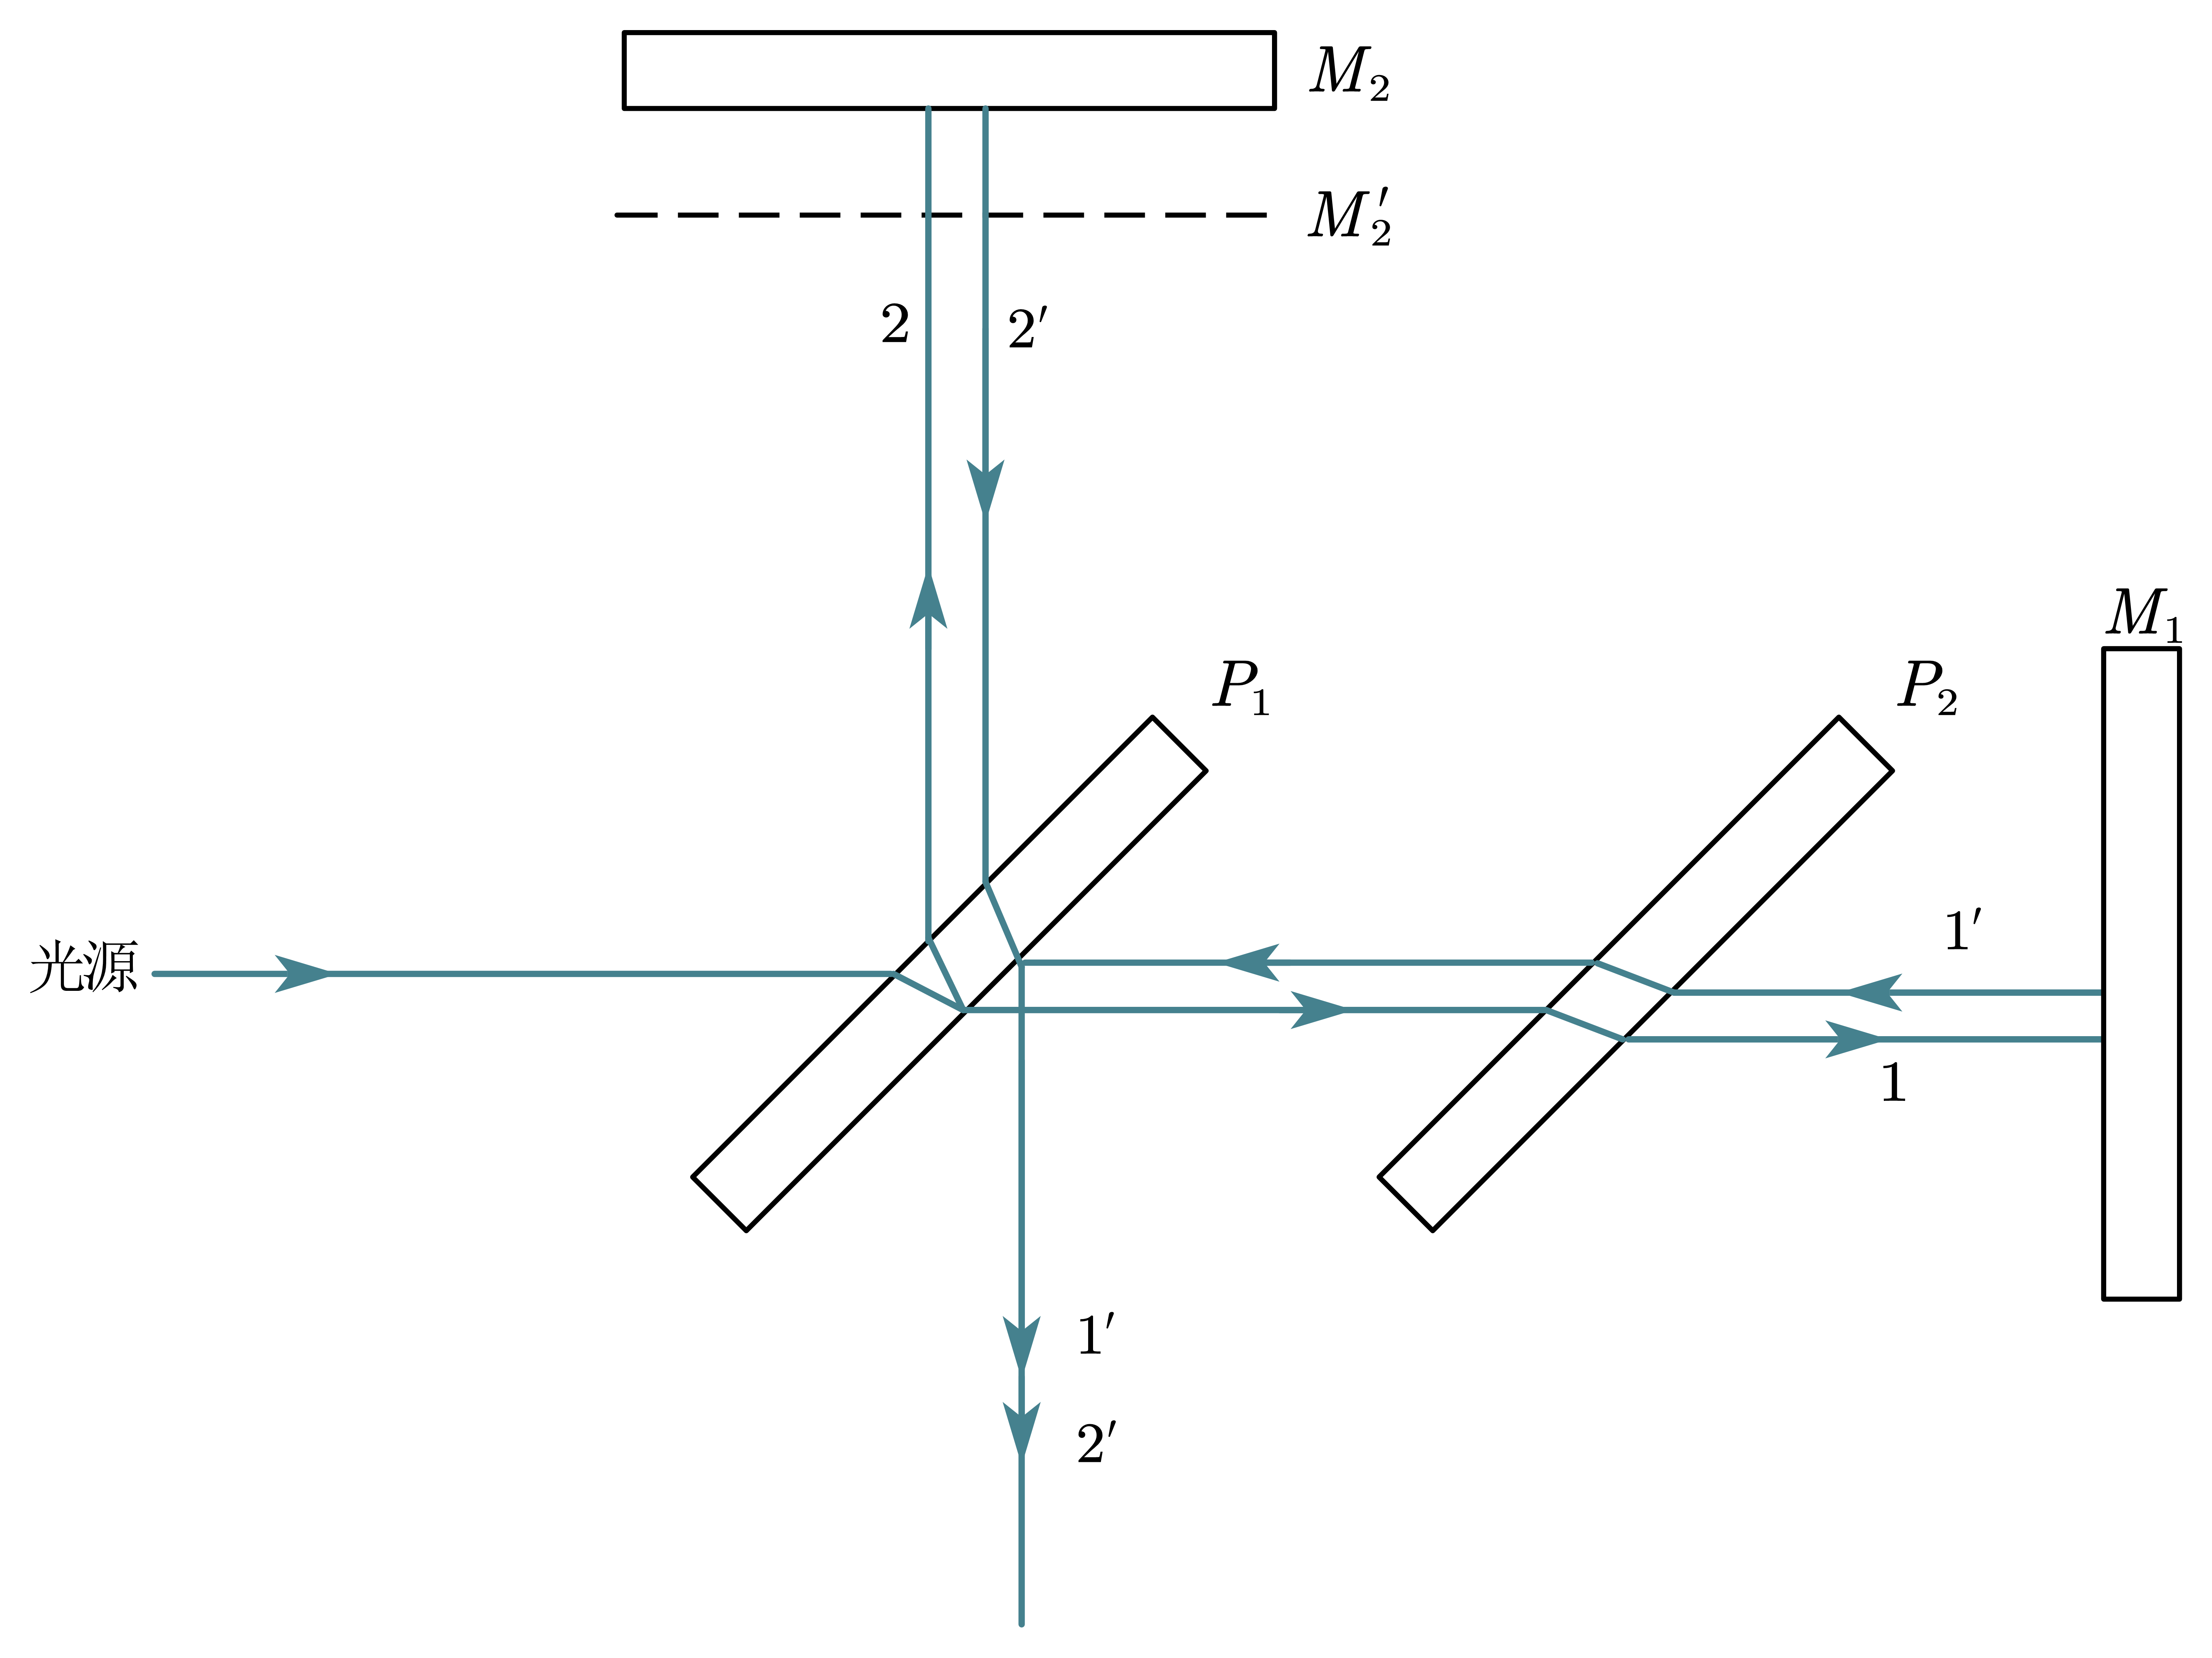
\includegraphics[width=0.5\textwidth]{迈克尔干涉仪原理.png}
	\caption{迈克尔孙干涉仪原理}
\end{figure}
\subsubsection*{条纹数量和d改变量的关系}
\[
	\delta d = N\frac{\lambda}{2}
\]
\subsection*{[实验内容]}
\subsubsection*{调节干涉仪,观察非定域干涉}
\par \textbf{一、水平调节}\quad 调节干涉仪底脚螺丝,使仪器导轨平面水平,然后用锁紧圈锁住。
\par \textbf{二、等臂调节}\quad 调节粗调手轮移动$M_2$镜,让$M_1,M_2$镜与分光板$G_1$,大致等距离。
\par \textbf{三、最亮点重合}\quad 打开激光开关,检查激光输出嘴的位置和方向,让光束垂直射向$M_1$的中心部位。将观察屏转向一侧并周定,戴上墨镜,直接观察$M_2$镜,视野 中呈现两排分别由$M_1$、$M_2$反射回来的亮点,找准每排亮点中最亮的那个点,分别调 节$M_1$和$M_2$两个反射镜背后的调节螺华(先调$M_1$再调$M_2$),使两排亮点中最亮的 光点严格重合,此时说明$M_1$已垂直$M_2$。注意调节时调节螺丝的松紧要均衡,防止损坏调节螺丝。
\par \textbf{四、条纹移到屏中央}\quad 将观察屏转回原位置,若上一步中的最亮点已经严格重合,则观察屏上可以观察到圆形干涉条纹,若没有条纹,可能是亮点没严格重合,或者条纹在屏幕边缘。调节粗调手轮使条纹大小、粗细适中,再轻微调节$M_1$,镜上的水平或竖直拉簧螺丝,使圆形条纹的中心位于屏中央。
\par \textbf{五、观察非定域干涉}\quad 前后左右移动屏的位置和角度,发现干涉条纹的大小或形状发生变化,证明非定义域干涉是空间处处相干的。
\par \textbf{六、条纹特征与$d$的关系} \quad 调节粗调手轮前后移动M2,观察条纹的“冒出”或“缩进”现象,判断M;与M之间的距离d是变大还是变小,并观察条纹的粗细、疏密和d之间的关系。

\subsubsection*{测量激光波长}
\par \textbf{一、仪器调零} \quad 因为旋转微调手轮时,粗调手轮随之变化,而旋转粗调手轮时
微调手轮并不随之变化,所以测量前必须调零。方法如下:沿某方向(例如顺时针)
将微调手轮调到零并记住旋转方向(为避免空程差,后面的测量都要沿此方向),沿
同一方向旋转粗调手轮使之对准某一刻度,注意此后粗调手轮不要再动。测量过
程中若需要反方向旋转微调手轮,则一定要重新调零。
\par \textbf{二、测量并计算波长} \quad 沿刚才的方向旋转微调手轮,条纹每冒出或缩进50个记录相应的M2的位置,连续记录6次以上,数据记录在表4-5-1中,用最小二乘法计算激光的波长。
\clearpage
\subsection*{数据处理}
\begin{figure}[!htbp]
	\centering
	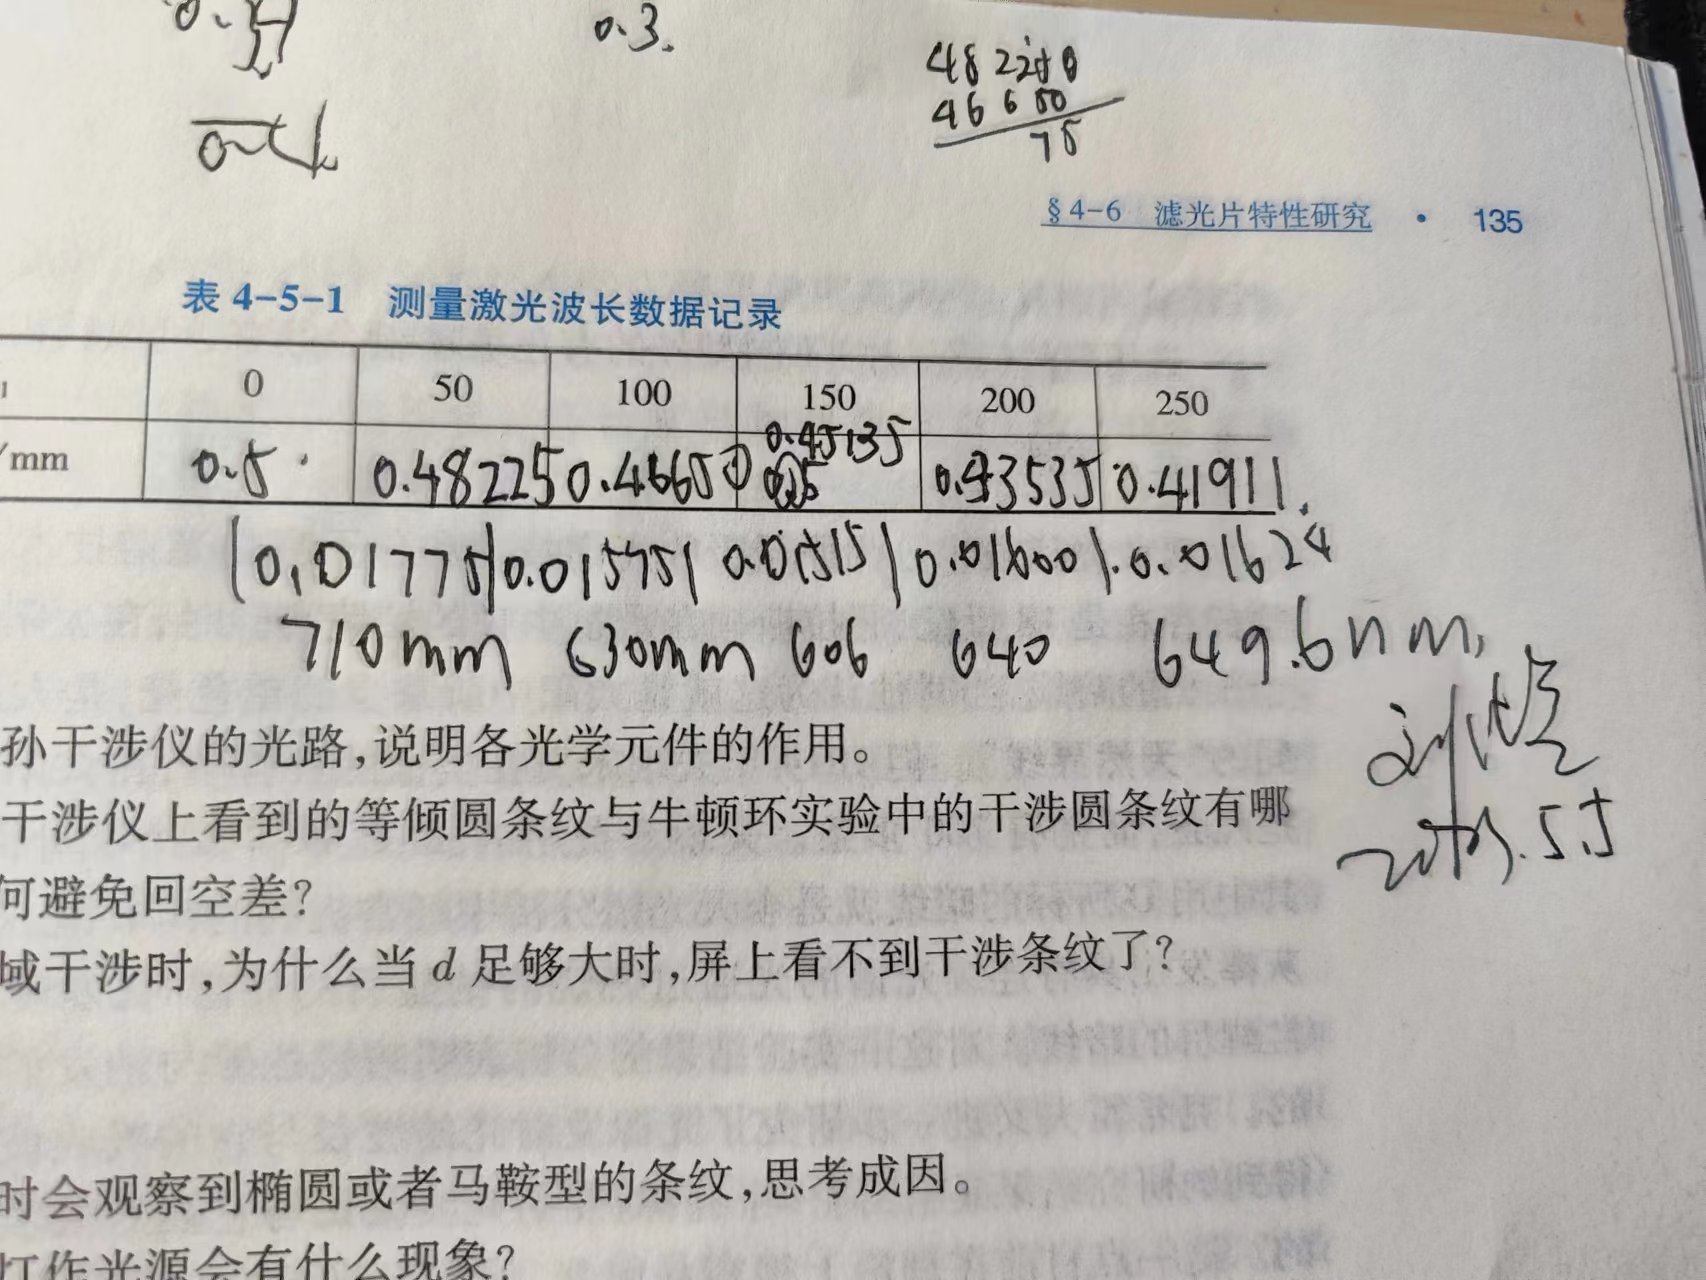
\includegraphics[width=0.8\textwidth]{实验数据.jpg}
	\caption{实验数据记录(带签名)}
\end{figure}
\begin{table}[!htbp]
	\centering
	\begin{tabular}{|c|c|c|c|c|c|}
		\hline
		计算次数 & 1 & 2 & 3 & 4 & 5 \\
		\hline
		数据 & 710nm & 630nm & 606nm & 640nm & 649nm \\
		\hline
		\end{tabular}
	\caption{实验数据记录}
		
\end{table}

\subsubsection*{使用最小二乘法计算波长}
\par 设激光的实际波长为$x$,为了减少误差,抛弃第一个数据,则只需要计算
\[
	\min{S(x) = (x-630)^2 + (x-606)^2 + (x-640)^2 + (x-649)^2} 
\]
\[
	S^{\prime}(x) = 2(x-630) + 2(x-606) + 2(x-640) + 2(x-649) = 8(x-631.25)
\]
\par 所以$x = 631.3$,即波长的估计值为$631.3nm$

\end{document}
